	 \areaset[0cm]{11.5cm}{27.4cm}
\section{The human cardiovascular system}\label{sec:CardiovascularSystem}
	
\subsection{The double circuit system}
		\begin{mdframed}[style=exampledefault, userdefinedwidth=16cm,					 frametitle={Starr chapter 33}\label{mat:BEISPIELMATERIAL}]	  
			A humingbird's heart makes up to 1500 beats per minute (bpm), whereas our heart won't make more than 200 bpm. In both cases the heart can't ever stop over a mammal's lifetime.  Starr \ding{229} 33.1 embraces the evolution of a double circuit system with \textbf{pulmonary circuit} and \textbf{systemic circuit}. Starr \ding{229} 33.2 covers this in greater detail.
		\end{mdframed}
		
\begin{enumerate}[leftmargin=*,series=chapter]
\item  Complete figure \ref{fig:KreislaufSchemaLeer}
 with aid of your biology book Starr \ding{229} 33.2. Check out \emph{figure} Starr 33.5 too! 
 Label \emph{1} through \emph{15} and \emph{a)} trough \emph{f)}. Colour the blood vessels accordingly \textbf{red} or \textbf{blue}. \textbf{ \ding{253} HW-assignment on moodle! }
\end{enumerate}


\Loesung{
\marginnote{
    \begin{tabularx}{5cm}[]{p{0.5cm} p{4.5cm}}
			\toprule
			No & term \\\midrule
			a) & capillaries of head and brain \\
			 b) & lungs \\
			c) & liver \\
			 d) & intestines \\
			e) & kidneys  \\
			 f) & legs \\
			1 & pulmonary veins \\
			2 & pulmonary arteries \\
			3 & left atrium  \\
			 4 & left ventricle \\
			 5 & hepatic arteries  \\
			6 & abdominal aorta /  \\
			7 & renal artery  \\
			8 & renal vein \\
			 9 & hepatic portal vein  \\
			10 & hepatic vein  \\
			11& inferior vena cava \\
			 12 & right ventricle \\
			13 & right atrium   \\
			14 & superior vena cava \\
			15 & carotid arteries \\
			\bottomrule
			\end{tabularx}%
			}}{0cm}
			
	\begin{minipage}{11.4cm}
		  \includegraphics[width=1\textwidth]{/images/biozone-human-0114-v3.png}
		  \captionof{figure}[Kreislauf verändert nach Biozone-Human]{Complete this scheme of the human cardiovascular system accordingly. \\[4pt] \textbf{hints}: \textit{Structure d) are the capillaries of the intestines; No 5 are hepatic arteries (not shown in the book)}}
		  \label{fig:KreislaufSchemaLeer}
	\end{minipage}
		
\marginnote{\caution[t][blue][The hepatic portal vein]{\ding{229} Starr figure \textbf{33.4}, label \kreis{6} and explain the role of the hepatic portal veine: \Loesung{\\ Most nutrients are transported from the intestines to the liver where they are either stored, processed or further moved on to the blood stream }{3cm}}}[-3cm]



	 \areaset[0cm]{16cm}{27.5cm} 
\subsection{Blood is live}\label{ssc:Blood}

		\begin{mdframed}[style=exampledefault, userdefinedwidth=16cm, frametitle={Starr chapter 33.4}\label{mat:BEISPIELMATERIAL}]	  
			This is an essential part of our syllabus and well covered in your text book.
		\end{mdframed}

	\begin{enumerate}[itemsep=1.5em, resume, leftmargin=*,series=chapter]
	\item Figure \ref{fig:BloodSummary} provides a summary on the composition of blood. Write short statements about structure and functions to each of the components! \textbf{ \ding{253} HW-assignment on moodle! }
	\label{task:BloodSummary}
	\end{enumerate}
	

\Ersatz{	
	\begin{minipage}[htbp]{16cm}
	\flushleft {\includegraphics[width=1\linewidth]{/images/figures/Russel-44_10-a.jpg}}   \captionof{figure}[composition of blood; Russel chp 44 pict 10-a]{\textbf{solution to:} Blood components and blood quantities in humans.}  	\label{fig:BloodSummary}
	\vspace{2pt}
	\end{minipage}
	}{%
	\begin{minipage}[htbp]{9cm}
	\flushleft {\includegraphics[width=1\linewidth]{/share/SB_Unterricht/Biologie/hum02_Gasaustausch/Blut/Blut-Uebersicht_v5.png}}   \captionof{figure}[Blutbestandteile aus Skript von Nora Lieske]{Blood components and blood quantities in humans.}  	\label{fig:BloodSummary}
	\vspace{2pt}
	\end{minipage}
	}
	
	
	
	
 \areaset[0cm]{11.5cm}{26.5cm}
% \clearpage
\subsection{What is the \emph{pulse} and how do you measure it?}

		\marginline{
			\textit{What you'll need: \begin{itemize}
		                           \item a stop watch to count your pulse
		                           \item Starr 33.6 (8ed) or 33.5 (9ed) to fill in the missing gaps
		                          \end{itemize}
					}}

\emph{What is the "`pulse"'?}  During ventricle \gapn{systole ...} blood is pumped out of the heart and travels as a wave through the aorta and the subsequent \gapn{arteries...}. This wave of blood bulges\sidenote{"`to widen"', \textit{wölben}} \gap{arteries ...} and this is what you can feel, when holding your \gap{fingers} on \gap{arteries ...} that run near the body \gap{surface ...}.  

Thus each heart beat produces a \gap{pulse ...}

And the pulse frequency corresponds with the \gap{heart beat frequency}

Your pulse may depend on your \gap{physical activities ...} or your \gap{mood}

Therefore, your pulse is an important indicator about the condition of the activity of your \gap{heart ...}.

Starr (p. 546, 8ed / p. 578, 9ed) explains you how to accurately measure your pulse - for example at the \gap{radial} artery of your arm: \Loesung{ For example, to feel the pulse in your radial artery put your fingers on your inner wrist near the base of your thumb}{3cm} - count for 30 sec. or even better for a full hour.
 


% 	 \begin{hanging}
% 	  Fragestellung: Die menschliche Herzschlagfrequenz (der Puls) verändert sich bei körperlicher Belastung. Wann und wie?
% 	   \end{hanging}
	   
   \marginline{
	\textbf{Feel your pulse}, problem and method:
		\begin{enumerate}[itemsep=2pt,label=\textit{\roman*)},series=roman]
		\item How is your pulse going to change during physical exercise?
		\item Measure the pulse of your partner as described above, than change the roles.
		\item Measure your pulse again, but now after 15 knee bends and then also after 30 knee bends
		\item  List your values in table  \ref{tab:PulsResultate}.
		\item Compare your values with those referenced in table \ref{tab:PulsNorm}
		\end{enumerate}
		}

	\begin{table}[!htbp]
	\setlength{\extrarowheight}{6pt}	
	\captionof{table}[eigene Resultate Puls]{Your measured pulse values:}
	  \vspace{12pt}  \hspace{0cm}
	    \begin{tabularx}{12cm}[]{X p{3cm} p{3cm}} %
	\toprule
	 Measurement after & Pulse of student A & Pulse of student B  \\\midrule
	  rest &  & \\
	 15 knee bends &  & \\
	 30 knee bends&  &   \\
	\bottomrule
	\end{tabularx}%
	  \label{tab:PulsResultate}%
	\end{table}% 


	\begin{table}[!htbp]
	\setlength{\extrarowheight}{4pt}	
	\captionof{table}[Normawerte Puls]{Norm values of the pulse at different ages:}
	  \vspace{12pt}  \hspace{0cm}
	    \begin{tabularx}{12cm}[]{X p{2cm}  | X p{2cm}} %
	\toprule
	 Age  & Pulse & ~ ~ Age & Pulse  \\\midrule
new bornes &  120-140  &  ~ ~toddlers &  120 \\
teenagers &  80 & ~ ~ adults &  60-80 \\
elderly &  70-90 &  ~ ~ maximum pulse & 200 \\
	\bottomrule
	\end{tabularx}%
	  \label{tab:PulsNorm}%
	\end{table}% 

		\begin{mdframed}[style=exampledefault, userdefinedwidth=16cm, frametitle={Starr chapters 33.5 and 33.6}\label{mat:BEISPIELMATERIAL}]	  
			You've now covered the chapters 33.5 and 33.6 which are part of the syllabus. Further training materials may be available at the end of chapter \ding{229}  Starr 33.
		\end{mdframed}
% \clearpage

\areaset[0cm]{16cm}{27.4cm}
\subsection{Capillaries and the formation of tissue fluid}\label{sec:CapillariesTissuefluid}

		\begin{mdframed}[style=exampledefault, userdefinedwidth=12cm, frametitle={Starr chapter 33.7}\label{mat:BEISPIELMATERIAL}]	  
			This chapter explains how cells are being provided with nutrients and oxygen even though many cells do not directly tap a blood vessel.
		\end{mdframed}



\begin{enumerate}[resume, leftmargin=*,series=chapter]
\item  There are no "`pumps"' to drive the exchange of fluids and solutes in and out of capillaries. Passive transport is due to \emph{osmosis} -  process you learned about two years ago, in grade three. Annotate and colour figure \ref{fig:CapillaryExchangeMarkl} to explain how osmosis drives the exchange of nutrients, gases and water in and out of capillaries!
\end{enumerate}

	\vspace{14pt}
\Ersatz{
	\begin{minipage}[htbp]{16cm}
	\centering {\includegraphics[width=1\linewidth]{/share/00_SCHULE_DATA-add/bilder_saz/Markl_Bilder/5_8_Stoffwechsel/5_Stoff_und_Energieaustausch_bei_Tieren/05_06_03_1_v2_en.png}} \captionof{figure}[Austausch von Stoffen an der Kapillare aus Markl 5.6]{Describe the processes indicated in this figure!}  	\label{fig:CapillaryExchangeMarkl}
	\end{minipage}
	}{
	\hspace{-3cm}
	\begin{minipage}[htbp]{16cm}
	\centering {\includegraphics[width=1\linewidth]{/share/00_SCHULE_DATA-add/bilder_saz/Markl_Bilder/5_8_Stoffwechsel/5_Stoff_und_Energieaustausch_bei_Tieren/05_06_03_1_v2.jpg}} \captionof{figure}[Austausch von Stoffen an der Kapillare aus Markl 5.6]{Describe the processes indicated in this figure!}  	\label{fig:CapillaryExchangeMarkl}
	\end{minipage}	
	}
	
\vfill	
\marginnote{\caution[c][orange][moodle]{find a film about this topic on \textsc{moodle}!}}[2cm]
	\vfill	

\clearpage
% TEXTimMDframed
\areaset[0cm]{14cm}{26.5cm}  
\subsection{Red blood cells and blood types}
		\vspace{-0.2cm}
Knowing your blood type is essential in case of a blood donation. 
\marginline{\Loesung{\href{/share/SB_Unterricht/Biologie/hum02_Gasaustausch/Blut/BlutTransfusion18Jhd_lis_HS12.jpg}{transfusion of blood, mid 19th century}}{0cm}}  

\subsubsection{The AB0 blood types}
	\fboxsep4mm\fbox{
		\begin{minipage}{14cm}
			Mixing blood samples taken from different person one can either observe complete mixing or the formation of blood clots ("`clumps"'). The latter phenomenon is known as the \emph{agglutination} of red blood cells, the erythrocytes. The Austrian physician Karl Landsteiner was the first to explain agglutination in 1901 - he assumed substances on the surface of the erythrocytes to be the cause of this process. Today we know these substances as \textbf{antigen A} und \textbf{antigen B}. Antigens are made of proteins and sugars, they swim in the cell membrane. The name "`antigen"' is a acronym of "`\textbf{anti}body \textbf{gen}erating agent"' - hence there are antibodies which fit like a key into the lock. There are four different blood types, A, B, AB and 0 (zero) which were described by Landsteiner. Nowadays many more blood type systems are known - for example the so called rhesus factor (rh) or also referred to as blood group \textbf{D}. Read Starr (8ed chapter 34.8; 9ed 34.7) for a further understanding of blood type antigens and antibodies!
		\end{minipage}
		}


\begin{minipage}{16cm}\vspace{1.8cm}
	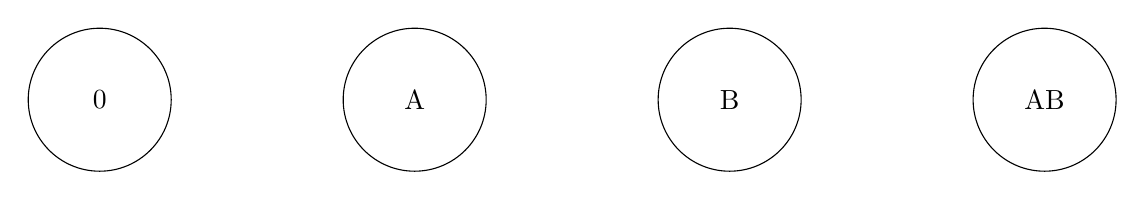
\begin{tikzpicture}[scale=1]
		\path[draw] (1,0) circle (6ex);\node at (1,0) {$0$};
		\path[draw] (5,0) circle (6ex);\node at (5,0) {A};
		\path[draw] (9,0) circle (6ex);\node at (9,0) {B};
		\path[draw] (13,0) circle (6ex);\node at (13,0) {AB};
	\end{tikzpicture}
	\vspace{2cm}
\end{minipage}



\vspace{0.4em}
\Kommentar{[Blutgruppen $A, B, AB, 0$ mit ihren Antigenen auf der Oberfläche]  }{}{0.8cm}{}

\vspace{0.3cm}
\enlargethispage{1.6cm}\hfill
\begin{minipage}[!h][][b]{12cm}
% % \setlength{\extrarowheight}{24pt} %% verträgt sich NICHT mit der Zentrierung
% \setcapmargin*[0cm]{0cm}
	\captionof{table}[Verzeichnis]{Punnet squar for the transfer of \textbf{blood} in the AB0-system \\ \textit{\textbf{remember:} There is NO "`universal donor"' for whole blood (serum \& cells) because when a transfer is done with whol blood, both antigens and antibodies must match! }}
	\begin{tabularx}{12cm}[]{m{2.2cm} | m{2.2cm} | m{2.2cm} | m{2.2cm} | m{2.2cm} m{0.1cm}  }% \toprule
	\textbf{Blut} & \centering \textbf{$0$} &\centering \textbf{A} &\centering \textbf{B} & \centering\textbf{AB}&   \\ [24pt] \midrule
	\textbf{$0$} &  & &  &  &  \\[24pt] \midrule
	\textbf{A}  &  & &  &   &  \\[24pt] \midrule
	\textbf{B} &  & &  & &  \\[24pt] \midrule
	\textbf{AB} &  & &  & &  \\[24pt] \midrule
	\end{tabularx}
\end{minipage}


%% I can't resume the list here - counter fails due to the dissection-counter (a workaround isn't trivial...)
% \ding{46} Copy the results from the blood typing test explained in \ding{229} Starr 34.7 (page 601) using the 8 circles below and write a short explanation about how this works!\label{exc:BloodTypeTheory}
%
%
% \vspace{0.6cm}
% 	\begin{tikzpicture}
% 		\path[draw] (1,0) circle (6ex);
% 		\path[draw] (5,0) circle (6ex);
% 		\path[draw] (10,0) circle (6ex);
% 		\path[draw] (14,0) circle (6ex);
% 	\end{tikzpicture}
% 	\vspace{0.3cm}
%
% 	\begin{tikzpicture}
% 		\path[draw] (1,0) circle (6ex);
% 		\path[draw] (5,0) circle (6ex);
% 		\path[draw] (10,0) circle (6ex);
% 		\path[draw] (14,0) circle (6ex);
% 	\end{tikzpicture}
%
% 	\vspace{2cm}
% \textbf{class activity:} Graphical explanation of antibodies and antigens:
% 		\vspace{1cm}
%
% 	\begin{tikzpicture}
% 		\path[draw] (1,0) circle (4ex);
% 		\path[draw] (5,0) circle (4ex);
% 		\path[draw] (10,0) circle (4ex);
% 		\path[draw] (14,0) circle (4ex);
% 	\end{tikzpicture}
%
% 	\vspace{2cm}



 \areaset[0cm]{14cm}{26.5cm}      
\subsubsection{Identify your own blood group and microsopy of red blood cells}
		\vspace{-0.6cm}
		\begin{center}
		 \fcolorbox{red}{Gray!20}{\parbox{14cm}{\centering
		\textbf{Taking a blood sample}     
		
		A drop of blood may transfer a sickness from one person to another! When working with blood, always do it the professional way!
		
		 \textit{Hint: in order to get your blood flowing \textbf{swing your arm} before pricking, in order to increase blood supply in your fingers.}
		}}
		\end{center}

		\marginpar{Until blood agglutination was understood most attempts to transfer blood between two persons failed. Since Landsteiner's discovery, Serum rich in antibodies can be used to test blood samples before donation: donor and recipient blood types must match!}

% \vspace{-0.6cm}
\paragraph{Materials:} Serum A; Serum B; Serum D; physiologische Kochsalzlösung (NaCl 0.9\%); 2 microscope slides tooth picks; blood lancets; swabs; disinfectant; paper towels; waist bin (jar with a plastic bag); cover slips; microscope
		\begin{enumerate}[label=\textit{(\arabic*)},leftmargin=1em,series=zaehler,itemsep=-2pt]
		      \item Get all your materials ready; mark the one microscope slide on the \textit{left} half with \textbf{A} and on the \textit{right} half with \textbf{B}; on the other slide you mark \textit{left} \textbf{D} and right \textbf{NaCl}

		      \item Use a swap and KODAN-disinfectant  in order to disinfect your finger.

		       \item Hold your hand against the table's surface and prick your finger with a \textsc{sterile} device and  \emph{immediately} press out those droplets!

		      \item You need four drops - two on each side of the two slides.

	              \item Trash the blood pricking tool. Use the your swap to sterilise your finger again, then trash the swab too.

		      \item Add one drop of \textbf{serum A }to the blood drop at the mark \emph{A}.
		      Add one drop of \textbf{serum B }to the blood drop at the mark \emph{B}.
		      Add one drop of \textbf{serum D }to the blood drop at the mark \emph{D}.
		      Add one drop of \textbf{NaCl 0.9\% }to the blood drop at the mark \emph{NaCl}.

		     \item Mix blood and serum - use a new tooth pick for each of the four tests (A, B, D, NaCl).

		     \item Can you observe \textbf{blood clumps}?  \gap{ yes: blood drop with serum A }
		      \item Compare your result with your sketches on page \pageref{exc:BloodTypeTheory}!
			      \begin{itemize}
			       \item your \texttt{A-B-0} blood group: \gap{\ldots A \ldots}
			       \item your D- or rhesus- blood group: \gap{\ldots D = Rh+ \ldots}
			      \end{itemize}
		      \item Trash your specimen (including the glass slides in the small bins!)
		\end{enumerate}
		
% \subsubsection{Red blood cells under the microscope}
% 		\begin{enumerate}[label=\textit{(\arabic*)},leftmargin=0em,series=zaehler]
% % 		      \item \sout{give a drop of blood onto a fresh slide}
% % 		      \item \sout{add a drop of 0.9\%  \ce{NaCl} }
% 		      \item observe one of your unclotted specimens from the AB0 test at 400x magnification
% 		      \item you may use Immersion oil and the 1000x mangification \textrightarrow~ clean the lenses afterwards!!
% 		      \item    if time allows: add a drop of strong salt solution (\textbf{ \ce{NaCl} 6\% }) to a specimen with unclotted blood and observe how osmosis produces misformed red blood cells
% 		\end{enumerate}
%

\vspace{0.5cm} \enlargethispage{1.6cm}
\Pointinghand\, Lets have a look at the "`universal donor"' of \textbf{blood cells} (table \ref{tab:Eryspende}) and the "`universal donor"' for \textbf{plasma} (table \ref{tab:Plasmaspende}):

\hspace{-2cm}
\begin{minipage}[!h][][b]{7.5cm}
	\captionof{table}[Verzeichnis]{Punnet squar for the transfer of \textbf{red blood cells} in the AB0-system } \label{tab:Eryspende}
	\begin{tabularx}{7.5cm}[]{m{1.4cm} | m{1.1cm} | m{1.1cm} | m{1.1cm} | m{1.1cm} m{0.1cm}  }% \toprule
	\textbf{Ery\-thro\-cyten} & \centering \textbf{$0$} &\centering \textbf{A} &\centering \textbf{B} & \centering\textbf{AB}&   \\ [6pt] \midrule
	\textbf{$0$} &  & &  &  &  \\[6pt] \midrule
	\textbf{A}  &  & &  &   &  \\[6pt] \midrule
	\textbf{B} &  & &  & &  \\[6pt] \midrule
	\textbf{AB} &  & &  & &  \\[6pt] \midrule
	\end{tabularx}
\end{minipage}
\hspace{1cm}
\begin{minipage}[!h][][b]{7.5cm}
	\captionof{table}[Verzeichnis]{Punnet squar for the transfer of \textbf{plasma} in the AB0-system} \label{tab:Plasmaspende}
	\begin{tabularx}{7.5cm}[]{m{1.4cm} | m{1.1cm} | m{1.1cm} | m{1.1cm} | m{1.1cm} m{0.1cm}  }% \toprule
	\textbf{Blut\-plasma} & \centering \textbf{$0$} &\centering \textbf{A} &\centering \textbf{B} & \centering\textbf{AB}&   \\ [6pt] \midrule
	\textbf{$0$} &  & &  &  &  \\[6pt] \midrule
	\textbf{A}  &  & &  &   &  \\[6pt] \midrule
	\textbf{B} &  & &  & &  \\[6pt] \midrule
	\textbf{AB} &  & &  & &  \\[6pt] \midrule
	\end{tabularx}
\end{minipage}


\begin{enumerate}[itemsep=1.5em, leftmargin=*]
\item  Why is every blood sample being divided into plasma and hematocrit?
	\Loesung{\\ In order help more patients with a single blood donation}{1cm}
\end{enumerate}

	 \areaset[0cm]{11.5cm}{27.4cm} %% (restore default)
